
\section{Testing}
\thispagestyle{plain}
System testing or software testing, falls into something that is called “Black-box testing”. This is a method of software testing, that investigates the functionality of the application, eg. what it does. It will not interfere with it's internal structure or workings. 

\subsection{Testing Procedure}

When you are about to conduct a test, you find a test-person. Then you tell them what the software is supposed to do and further give them the Test cases[7.2]. It is very important for the test subjects to think loud so we can get maximum feedback from the testing. 

\subsection{Test Cases}

Test cases are built around the specifications and requirements of the application. What the application is supposed to do.  

\begin{table}[htp]
\begin{center}
\begin{tabular}{ i{4cm} ||  i{10cm}} \toprule
\multicolumn{2}{c}{\textbf{Get Places}} \\ \hline
ID & T-F1 \\ \hline
Requirements & SF-1 \\ \hline
Feature& Places are shown on the map \\ \hline
Preconditions& \begin{enumerate} \item Flickr is up \item The Flickr group contains photos with locations \item Application is installed on device \item Device is connected to the internet \end{enumerate} \\ \hline
Test Description& \begin{enumerate} \item Open the application \item Wait for 30 seconds \item Click on a pinpoint \item Zoom out to a world view  \end{enumerate} \\ \hline
Expected result & The map should show some clickable pinpoints. When clicked the pinpoints should open a little box containing a thumbnail picture and small text provided by the Flickr Stedr group. \newline
When zoomed out new places should be loaded according to what the user see. \\ \hline
Pass/Fail criteria & The test is considered a pass if the expected result happens. The last step that need to be passed is that the place at Grenada is shown. \newline
If there are any inconsistencies with the expected result, the test should be considered a fail. \\ \hline
Severity & High\\ \bottomrule
\end{tabular}
\end{center}
\caption{Test Case: Get Places}
\label{tab:Test Case: Get Places}
\end{table}


\begin{table}[htp]
\begin{center}
\begin{tabular}{ i{4cm} ||  i{10cm}} \toprule
\multicolumn{2}{c}{\textbf{Open menu}} \\ \hline
ID & T-F2 \\ \hline
Requirements & SF-2 \\ \hline
Feature& Drawer menu with options is opened. \\ \hline
Preconditions& \begin{enumerate} \item[ ]1,2,3,4 \end{enumerate} \\ \hline
Test Description& \begin{enumerate} \item Click on the menu button \item Click on all of the icons in the menu \item Click on the menu again \end{enumerate} \\ \hline
Expected result & When the menu button is pressed, a drawer menu should open. All of the icons in the drawer menu is also buttons and when clicked again, the menu button should close the drawer menu. \\ \hline
Pass/Fail criteria & The test is considered a pass if the menu button opens and closes a drawer menu. Also, all of the icons should \\ \hline
Severity & High\\ \bottomrule
\end{tabular}
\end{center}
\caption{Test Case: Open Menu}
\label{tab:Test Case: Open Menu}
\end{table}


\begin{table}[htp]
\begin{center}
\begin{tabular}{ i{4cm} ||  i{10cm}} \toprule
\multicolumn{2}{c}{\textbf{Views}} \\ \hline
ID & T-F3 \\ \hline
Requirements & SF-6 \\ \hline
Feature& All the views are accessible \\ \hline
Preconditions& \begin{enumerate} \item[ ]1,2,3,4 \item[T-F1] Get places \end{enumerate} \\ \hline
Test Description& \begin{enumerate} \item Click on a pinpoint \item Click on the small window that appears \item Click on one of the buttons \textit{Images, Sound, Story} \item Dependent on the previous step, click on the buttons not yet pushed \item Click the menu button \item Click home \end{enumerate} \\ \hline
Expected result & Which view that is selected is shown to the user by being in a different colour than the two other buttons. If the button for the selected view is touched, nothing should happen. \newline
For every button representing a non-selected view, the user should be taken to the view as indicated by the button text. \\ \hline
Pass/Fail criteria &The test is passed if the button: \newline[5pt]
Image - Takes you to the image view\newline
Story - Takes you to the story view\newline
Sound - Takes you to the sound view.\newline[5pt]
The selected view has a unclickable button in a different colour representing the selected view.\newline
Considered a fail if there are any inconsistencies with the criteria above. \\ \hline
Severity & High\\ \bottomrule
\end{tabular}
\end{center}
\caption{Test Case:  Views}
\label{tab:Test Case: Views}
\end{table}


\begin{table}[htp]
\begin{center}
\begin{tabular}{ i{4cm} ||  i{10cm}} \toprule
\multicolumn{2}{c}{\textbf{Load Content}} \\ \hline
ID & T-F4 \\ \hline
Requirements & SF-7 \\ \hline
Feature& Content is loaded for the places \\ \hline
Preconditions& \begin{enumerate} \item[T-F3] Views \end{enumerate} \\ \hline
Test Description& \begin{enumerate} \item Click on a pinpoint(not Camera Obscura) \item Click on the description \item Go through the views as in T-F3 \item[3a] Click on all of the titles on the story \item[3b] Click on two random images \item[3c] Click on a sound \end{enumerate} \\ \hline
Expected result & The places should be loaded with relevant and accessible content from all of the content providers.. \newline
If some content-types are not provided for the specific place, the content type should be loaded but indicate that it is empty. \\ \hline
Pass/Fail criteria &The test is considered a pass if the expected result happens. \newline
If there are any inconsistencies with the expected result, the test should be considered a fail. \\ \hline
Severity & High\\ \bottomrule
\end{tabular}
\end{center}
\caption{Test Case: Load Content}
\label{tab:Test Case: Load Content}
\end{table}



\begin{table}[htp]
\begin{center}
\begin{tabular}{ i{4cm} ||  i{10cm}} \toprule
\multicolumn{2}{c}{\textbf{Collection view}} \\ \hline
ID & T-F5 \\ \hline
Requirements & SF-8 \\ \hline
Feature& Show a view with the stories related to a collection \\ \hline
Preconditions& \begin{enumerate} \item[T-F2] Open menu \item[T-F4] Load Content \item[5] It exist a collection \end{enumerate} \\ \hline
Test Description& \begin{enumerate} \item Press the menu button \item Press the Collection button \item Press a collection \end{enumerate} \\ \hline
Expected result & When the collection button is pressed a new view should open with the list of stories related to the collection. \\ \hline
Pass/Fail criteria & The test is considered a pass if it is possible to open the menu and access a collection with a list of stories. \\ \hline
Severity & Medium\\ \bottomrule
\end{tabular}
\end{center}
\caption{Test Case: Collection View}
\label{tab:Test Case: Collection View}
\end{table}


\begin{table}[htp]
\begin{center}
\begin{tabular}{ i{4cm} ||  i{10cm}} \toprule
\multicolumn{2}{c}{\textbf{Collection map view}} \\ \hline
ID & T-F6 \\ \hline
Requirements & SF-8 \\ \hline
Feature& Show places related to a collection as pinpoints in a map \\ \hline
Preconditions& \begin{enumerate} \item[T-F2] Collection View \end{enumerate} \\ \hline
Test Description& \begin{enumerate} \item Press the menu button \item Press the Collection button \item Press a collection \item Press the \textit{show on map}-button \end{enumerate} \\ \hline
Expected result &When the “show on map”-button is clicked, a map view should open with related places showed as pinpoints. Pinpoints not related to the collection should not be placed on the map. \\ \hline
Pass/Fail criteria & The test is considered a pass if all places related to a collection is exclusively shown in a map view. \\ \hline
Severity & Medium\\ \bottomrule
\end{tabular}
\end{center}
\caption{Test Case: Collect Map View}
\label{tab:Test Case: Collect Map View}
\end{table}


\begin{table}[htp]
\begin{center}
\begin{tabular}{ i{4cm} ||  i{10cm}} \toprule
\multicolumn{2}{c}{\textbf{Gallery}} \\ \hline
ID & T-F7 \\ \hline
Requirements &  \\ \hline
Feature& Gallery function\\ \hline
Preconditions& \begin{enumerate} \item[T-F4] Load Content \item[ ] The application is in a place with a story where there are multiple images to the story. \end{enumerate} \\ \hline
Test Description& \begin{enumerate} \item Press the story title \item If there are more pictures related to a story, press the arrows \end{enumerate} \\ \hline
Expected result &When accessing stories with multiple pictures as content, arrows indicating the possibility to go through picture files should appear. When pressed new images should replace the old picture. \\ \hline
Pass/Fail criteria &The test is considered a pass if the expected result happens. \newline
If there are any inconsistencies with the expected result, the test should be considered a fail. \\ \hline
Severity & Low\\ \bottomrule
\end{tabular}
\end{center}
\caption{Test Case: Gallery}
\label{tab:Test Case: Gallery}
\end{table}


\begin{table}[htp]
\begin{center}
\begin{tabular}{ i{4cm} ||  i{10cm}} \toprule
\multicolumn{2}{c}{\textbf{Upload Content}} \\ \hline
ID & T-F8 \\ \hline
Requirements &  SF-9\\ \hline
Feature& Content can be uploaded to Instagram, Twitter and SoundCloud \\ \hline
Preconditions& \begin{enumerate} \item[T-F4] Load Content \item[6] Successfully connected to the content (not story provider) providers \end{enumerate} \\ \hline
Test Description& \begin{enumerate} \item Click on a pinpoint \item Click on the description \item Go through the views as in T-F3 \item Upload textual content to Twitter \item Upload picture to Instagram \item Upload sound to SoundCloud \end{enumerate} \\ \hline
Expected result &The places should be loaded with relevant and accessible content from all of the content providers..\newline
If some content-types are not provided for the specific place, the content type should be loaded but indicate that it is empty. \\ \hline
Pass/Fail criteria & The test is considered a pass if the expected result happens. \newline
If there are any inconsistencies with the expected result, the test should be considered a fail. \\ \hline
Severity & Medium\\ \bottomrule
\end{tabular}
\end{center}
\caption{Test Case: Upload Content}
\label{tab:Test Case: Upload Content}
\end{table}

\clearpage

\subsection{Test Execution}
\label{sec:TestExecution}
\subsubsection{System Testing}

During the final stages of the development, it was performed a system test after integrating all of the developed components. This was an important step done before the acceptance testing, to see that all of the components developed by different team members and the former development team worked together. Since we did not have the resources it was impossible to let an external team do the testing, but to emulate some sort of indipendence to the system the tests were done by a group member who had been less involved in the development of the client and never tried the client on a smartphone. This of course is a weakness in the testing, since the tester had a general knowledge of the system worked and also a basic idea of the client from using the system on a smartphone emulator.

A summary of the test results is shown in the table below, and an example from the test log can be found in the appendix.

\begin{table}[!htp]
\begin{center}
	\begin{tabular}{ | l | l | l | }
	\hline
	 \ID	 	& Pass 		& Comment 	\\ \hline
	T-F1		&Unknown		& Valid with full cache, not valid when empty cache	\\ \hline
	T-F2		&Pass		& None	\\ \hline
	T-F3		&Pass		& None	\\ \hline
	T-F4		&Pass		& None	\\ \hline
	T-F5		&Pass		& None 	\\ \hline
	T-F6		&Pass		& None 	\\ \hline
	T-F7		&Pass		& None 	\\ \hline
	T-F6		&Fail			& This feature was declared infeasible  	\\ 
	 \hline
 	 \end{tabular}
\end{center}
\caption{System Testing: Validity}
\label{tab:System Testing: Validity}
\end{table}

\subsubsection{Acceptance Testing}

Acceptance testing is one of the last levels of the software testing process. The purpose of such testing is to evaluate the system's compliance with the given requirements to check whether it is acceptable for delivery. Hence the name acceptance testing.

On May 14. during one of our last meetings we sat down with Jaqueline Floch for the final acceptance test of our system. This acceptance test included further developed features and improvements of the graphical user interface.

For the main test we had a feature based acceptance test where we went through the requirement list. Not to say that usability is not as important, but our customer had received the latest build almost every week in the later stages of the project. With this, the customer have conducted usability acceptance testing regularly throughout the project, giving us feedback. Because of this we did not have the same need for a usability based user acceptance test, which we know is the norm, but Jaqueline Floch had the app tested by four of her colleagues, which all gave positive feedback. If there had been any crucial shortcomings it probably would have been pointed out.

The test was conducted by going through the requirement list sorted by priority and individually receiving a verdict on acceptance. The individual requirement either reviewed \texttt{Pass, fail, outdated} or \texttt{cancel} if the requirement was withdrawn. The latter was the case on a lot of the requirements with lower priority since we had little time and the customer wanted us to focus on the more important tasks.

The result of the acceptance test are listed below:\\

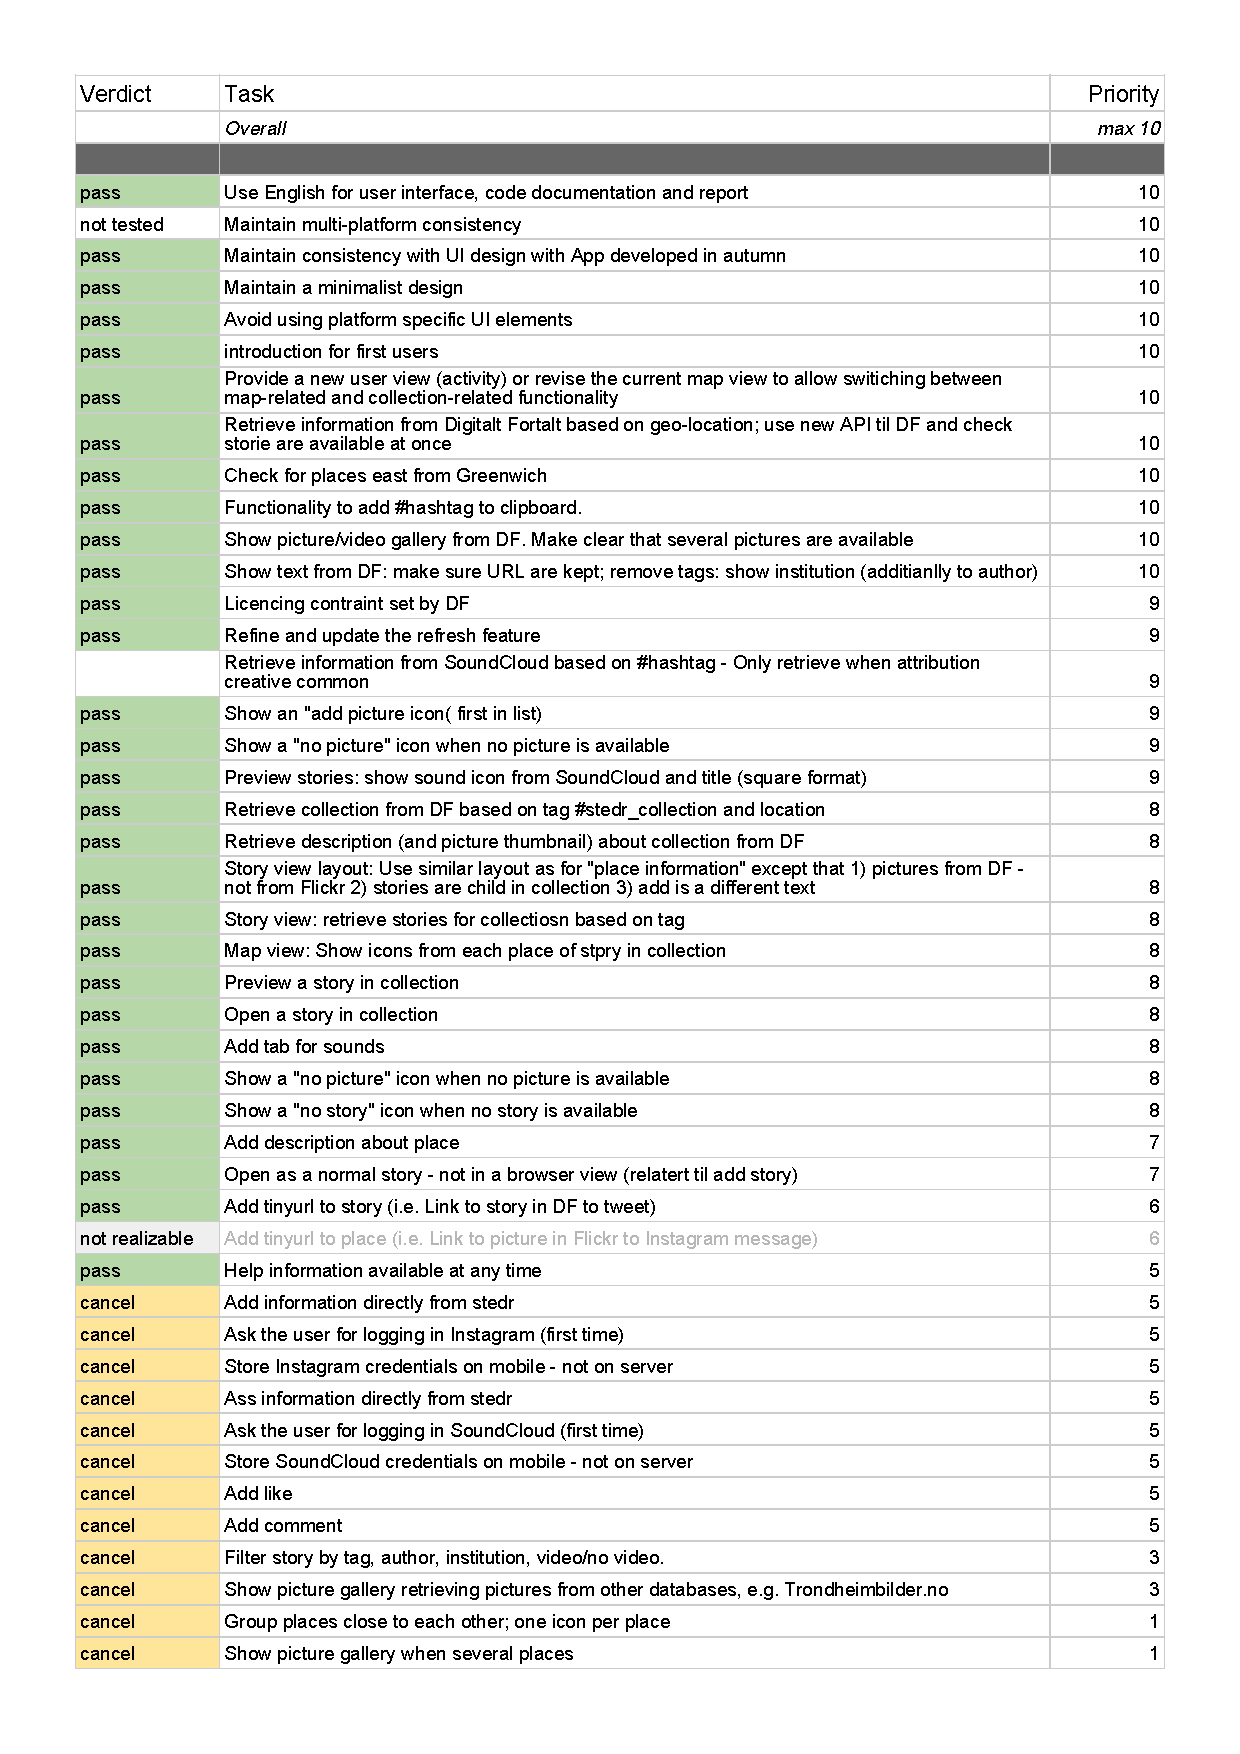
\includepdf[%
 	pages={-},
	offset=0in 0in,%
	]{res/AcceptanceTesting_Requirements.pdf}
\label{sec:featList}
As you can see, one requirement are missing a verdict. This is is because this was not testable since we waited for a response from SoundCloud at the time. This was later implemented and are now working as it should.


\subsubsection{NFR testing}
It is important for the project that our result meets the projects main non-functional requirements, described in the ``Product quality'' section of the SRS chapter (\ref{sec:ProductQuality}), for it to be considered a success. 

\paragraph{Compability}

\emph{Co-existence}
With the result found under Reliability - maturity, it is clear that the system can handle that multiple client share the same environment. It is worth to notice that the testing program makes use of threads to be more realistic regarding parallel requests to the server.

\emph{Interoperability}
Since the requirement for interoperability was said to be fulfilled as long as the system followed a standardized method of communication over a known and widely used protocol, the testing consisted of looking at the objects sent from the server and acknowledge that they were valid JSON-objects.

\begin{table}[!htp]
\begin{center}
	\begin{tabular}{ | l | l | l | }
	\hline
	 \#	 	& Content 		& JSON 	\\ \hline
	 1		&Places		& Yes	\\ \hline
	 2		&Stories		& Yes	\\ \hline
	 3		&Images		& Yes	\\ \hline
	 4		&Collections	& Yes	\\ \hline
	 5		&Sound		& Yes 	\\
	 \hline
 	 \end{tabular}
\end{center}
\caption{Compability: Interoperability}
\label{tab:Compability: Interoperability}
\end{table}

\paragraph{Performance Efficiency}
We have greatly improved the core of the system to boost the efficiency of the application. This should cause the application to use no more than 300 seconds to pull new content from the APIs. The efficiency was tested by adding new content and recording 10 times with different content posted at different times. By measuring the individual response times and calculating the average result we will get a rough estimate.\\

\begin{table}[!htp]
\begin{center}
	\begin{tabular}{ | l | l | l | r | }
	\hline
	 \#	 	& Content 		& Time a day 		& Result \\ \hline
	 1		&Instagram		& 10:55			& \texttt{1 sec} \\ \hline
	 2		&Instagram		& 14:40			& \texttt{1 sec} \\ \hline
	 3		&Instagram		& 14:45			& \texttt{1 sec} \\ \hline
	 4		&Tweet		& 14:16			& \texttt{19 sec} \\ \hline
	 5		&Tweet		& 14:18			& \texttt{20 sec} \\ \hline
	 6		&Tweet		& 10:40			& \texttt{20 sec} \\ \hline
	 7		&Story		& 15:26			& \texttt{133 sec}\\ \hline
	 8		&Story		& 16:15			& \texttt{10 sec}\\ \hline
	 9		&Story 		& 11:00			& \texttt{104 sec}\\ \hline
	 10		&Story		& 15:48			& \texttt{135 sec}\\ \hline
	 11		&Story		& 16:03			& \texttt{107 sec}\\ \hline
	 13		&Story		& 19:01			& \texttt{132 sec}\\ \hline
	 14		&SoundCloud		& 18:51			& \texttt{5 sec}\\ \hline
	 15		&SoundCloud		& 19:15			& \texttt{7 sec}\\ \hline
	 16		&SoundCloud		& 19:20			& \texttt{6 sec}\\  
	 \hline
 	 \end{tabular}
\end{center}
\caption{Performance Efficiency: Publishing New Content}
\label{tab:Performance Efficiency: Publishing New Content}
\end{table}

Since much of the test content had relatively consistent results we did not think more testing was needed. The Instagram images appeared almost instantly ( 1 second) consistently, since we completed the tests manually, we could not measure finer times. The twitter content were a little slower as expected, but did also appear consistently at a reasonable time averaging in just under 20 seconds. The SoundCloud publishing also happened pretty quick averaging \texttt{6 seconds} As for the stories we published through Digitalt Fortalt, the times were very inconsistent. In three of the tests (\# 7, \#10 and \#12), which was the longest ones, the content had to be uploaded to DF as well as being published. This probably added to the time. All the other tests were performed with the content already uploaded, but we still recorded a massive variation in results ranging from \texttt{10 seconds} (\#8) to \texttt{105 seconds} (\#9).


Average: 
\begin{equation}
\frac{133 + 10 + 104 + 135 + 107 + 132}{6} = {103.5}
\end{equation}

With all results clocking in under 150 seconds, and our goal being under 300 seconds, we are very pleased with the results and can happily see our app passing this test. Considering that the original app needed multiple days for the results to appear, it is needless to say that there have been a massive improvement.


Another important part of the performance efficiency is the application's data usage. Blowing the users' data limit and potentially taking a large part in increasing their phone-bill is something we want to avoid. To avoid this we have implemented a data usage restraint. This restraint is set through equation (\ref{eq:DownloadLimit}) in section \ref{sec:ProductQuality}.

We tested the data usage to make sure our application met our standard. We measured this roaming unconnected to any WiFi-hotspots while running the app.\\

\emph{Quick session}\\
Opening map: \texttt{55.74 kB}\\
Entering place with only one story: \texttt{+ 6.07 kB}

\emph{Browsing session}\\
Browsing map over Trondheim: \texttt{1.64 MB}\\
Entering place with 6 stories and 2 Instagram pictures: \texttt{+ 0.02 MB}

We found these results to be pretty reasonable. The app does not download more content than necessary, and the results seems really consistent compared to the experiences we have had using the previous application.

\paragraph{Reliability}

Testing of components was done by feeding test cases to the components. When accepted, these new components was added to a running server instance that acted as a beta. The beta server was deployed at the 9th of April and has since been monitored to record uptime and errors. Shortly after Easter the old server was changed with the new one so that the customer could use new features, but also so that it was possible to monitor how the server performed under normal usage.

A shortcoming to the test-data below is that each time new features was deployed to the server, the server was restarted. Because of this, the longest interval the server has been running uninterrupted is approximately one week. 

\emph{Maturity}\\
The testing of maturity was done by analysing the data recorded in comparison to the feedback we got from the customer. Also, there was done an additional test where specific task were completed. Since maturity considers the system under normal use, the additional test was not a stress test in terms of using the system until it broke. Rather it was using the system at a relatively high frequency and noting the number of incidents.

To simulate users we made a testing program which made a total of 500 requests over a short period of time ($<5 minutes$). This test was done eight times over a single day, but with random rest periods for the server. If the server returned an error this was noted. 

\begin{table}[!htp]
\begin{center}
	\begin{tabular}{ | l | l | l | p{7cm} | }
	\hline
	\#	&Time since last test &Number of errors	& Notes \\ \hline
	1	&NA			& 1 & Places do not load. This also disables all other content retrievers\\ \hline
	2	&30 minutes		& 0 & Stories do not load. Does not affect other parts of the system\\ \hline
	3	&60 minutes		& 1 & Instagram pictures do not load. Does not affect other parts of the system\\ \hline
	4	&10 minutes		& 0 & Sounds do not load. Does not affect other parts of the system\\ \hline
	5	&120 minutes	& 1 & Total systems fail\\ \hline
	6	&60 minutes		& 1 & Places do not load. This also disables all other content retrievers\\ \hline
	7	&10 minutes		& 0 & Stories do not load. Does not affect other parts of the system\\ \hline
	8	&60 minutes		& 1 & Instagram pictures do not load. Does not affect other parts of the system\\
	 \hline
	 \end{tabular}
\end{center}
\caption{Maturity Testing}
\label{tab:Maturity Testing}
\end{table}

The test results clearly shows that there is a problem when the server has been inactive for more than an hour. This is because the server keeps a cache of places for an hour, before it deletes the cache. After the cache is emptied the server waits for a request before it again repopulates the cache. Also, when the server requests Flickr for new places it throws a time-out error. The time-out error doesn't have an effect for the user other than that the application is a bit slow if the user is the first to use the system after the cache has been emptied.

\emph{Availability}\\
Since the customer started using the new server (23rd of April) the server has been functional continuous, except from the 6th to the 7th of May. This gives that the system has had an uptime under presumably normal use of:

$1-\frac{24 hrs}{23 days \times 24 hours} \times 100 = 95.652 \% $

\emph{Fault tolerance}\\
The systems fail noted under the availability test was due to an global error on one of the systems external system. From this it is clear that the system depends totally on some of it's components and thereby external systems to provide the required functions. To determine how many critical components that exists in the systems, every component in the system was disabled to see the effect on the system. In addition, another part of the test considered interrupting connections to external systems. 

Note that to be considered functional, the system had to show places and load stories to the end-user. 

\begin{table}[!htp]
\begin{center}
	\begin{tabular}{ | l | p{4.2cm} | l | p{6.5cm} | }
	\hline
	\#	&Disabled Component	&Functional system	& Notes \\ \hline
	1	&Flickr Retriever		&No			& Places do not load. This also disables all other content retrievers\\ \hline
	2	&Story Retriever		&No			& Stories do not load. Does not affect other parts of the system\\ \hline
	3	&Picture Retriever	&Yes			& Instagram pictures do not load. Does not affect other parts of the system\\ \hline
	4	&Sound Retriever	&Yes			& Sounds do not load. Does not affect other parts of the system\\ \hline
	5	&External component (Heroku)	&No			& Total systems fail\\ \hline
	6	&External component (Flickr)	&No			& Places do not load. This also disables all other content retrievers\\ \hline
	7	&External component (Digitalt Museum)	&No		& Stories do not load. Does not affect other parts of the system\\ \hline
	8	&External component (Instagram)	&Yes			& Instagram pictures do not load. Does not affect other parts of the system\\ \hline
	9	&External component (Soundcloud)	&Yes			& Sounds do not load. Does not affect other parts of the system\\ 
	 \hline
	 \end{tabular}
\end{center}
\caption{Fault Tolerance Testing}
\label{tab:Fault Tolerance Testing}
\end{table}

This describes a major drawback of the reliability of the system, out of the four retrievers there are two single points of failure. In addition, the system also depends on three of five external systems to function properly. It is also important to note that if any of the external systems make radical changes so the system components becomes outdated, this will also lead to a non-functional system. Because of this the system cannot say to satisfy the requirement for fault tolerance.

\emph{Recoverability}\\

Testing for recoverability was done together with the testing for fault tolerance, by taking the time on how long it took for the system to be functional after re-enabling an external or internal components. Since the system isn't a critical system, the timing requirement was set to five minutes, so to pass the recoverability requirement the system should function normally within five minutes of the component re-enabling. 

\begin{table}[!htp]
\begin{center}
	\begin{tabular}{ | l | l | p{3.7cm} | r | }
	\hline
	\#	&Disabled Component	&Functional system  after five minutes	& Notes \\ \hline
	1	&Flickr Retriever		&Yes			& $<5 minutes$ \\ \hline
	2	&Story Retriever		&Yes			& $<5 minutes$\\ \hline
	3	&Picture Retriever	&Yes			& $<5 minutes$\\ \hline
	4	&Sound Retriever	&Yes			& $<5 minutes$\\ \hline
	5	&External component (Heroku)	&Yes			& $<5 minutes$\\ \hline
	6	&External component (Flickr)	&No			& $<60 minutes$\\ \hline
	7	&External component (Digitalt Museum)	&Yes		& $<5 minutes$\\ \hline
	8	&External component (Instagram)	&Yes			& $<5 minutes$\\ \hline
	9	&External component (SoundCloud)	&Yes			& $<5 minutes$\\ \hline
	 \hline
	 \end{tabular}
\end{center}
\caption{Recoverability Testing}
\label{tab:Recoverability Testing}
\end{table}

Because of a cache used to store places provided by Flickr, the system uses up to 60 minutes to refresh the cache. This means that errors so that Flickr doesn't respond to requests, leaves the system with an empty cache and thereby no places. This will again lead to a failure of the FlickrRetriver and the system itself as describes under the Fault Tolerance Test. 

\paragraph{Portability}

The multiplatform aspect of the project has played a major part in the development and have a large part in our choice of environment and frameworks. What we want to achieve is a reasonable consistency through different platforms and versions. We have throughout the development process tested it with many different virtual devices on different settings, but the most valuable ones are the ones performed on the physical devices at our disposal.\\

\begin{table}[!htp]
\begin{center}
	\begin{tabular}{ | l | l | l | r | }
	\hline
	 \#	& Platform (version)			&Device					& Notes \\ \hline
	 1	&Android (4.4.2 KitKat)			&LG Nexus 5 (3 different devices)	& Works fine\\ \hline
	 2	&Android (4.1 Jelly Bean)			&Samsung Galaxy SII			& Works fine\\ \hline
	 3	&Android (4.3 Jelly Bean)			&Samsung Galaxy Nexus			& Works fine\\ \hline
	 4	&Android (4.2 Jelly Bean)			&HTC One					& Works fine\\ \hline
	 5	&Android (4.0 Ice Cream Sandwich)	&Huawei Mediapad tablet			& Works fine\\ \hline
	 6	&Android (4.3 Jelly Bean)			&Sony Xperia Z1				& Works fine\\
	 \hline
	 \end{tabular}
\end{center}
\caption{Portability Testing}
\label{tab:Portability Testing}
\end{table}
